
\documentclass[12pt,twocolumn]{article}

\usepackage{graphicx}
\usepackage[none]{hyphenat}
\usepackage{listings}
\usepackage[english]{babel}
\usepackage{caption}
\usepackage{hyperref}
\usepackage{booktabs}
\usepackage{array}
\usepackage{amsmath}
\usepackage{fancyhdr}

\setlength{\headheight}{40pt}
\pagestyle{fancy}
\fancyhf{} % clear header and footer

\fancyhead[L]{%
  
\includegraphics[height=1.2cm]{Logo.png}
}

\fancyhead[R]{%
  \begin{tabular}{r}
    \textbf{Name:} Charan Kora \\
    \textbf{ID:} COMETFWC049 \\
    \textbf{Date:} 30-01-26
  \end{tabular}
}

\lstset{
  frame=single,
  breaklines=true
}

\newcommand{\mydet}[1]{\ensuremath{\begin{vmatrix}#1\end{vmatrix}}}
\providecommand{\brak}[1]{\ensuremath{\left(#1\right)}}
\providecommand{\norm}[1]{\left\lVert#1\right\rVert}
\newcommand{\solution}{\noindent \textbf{Solution: }}
\newcommand{\myvec}[1]{\ensuremath{\begin{pmatrix}#1\end{pmatrix}}}
\let\vec\mathbf

\graphicspath{{images/}}

\begin{document}

\begin{center}
\textbf{\large MATHEMATICS}
\end{center}

\section*{SECTION A}

\begin{enumerate}
\item In Fig., $PQ$ is a tangent at point $C$ to a circle with centre $O$. If $AB$ is a diameter and $\angle CAB = 30^\circ$, find $\angle PCA$.

\begin{center}
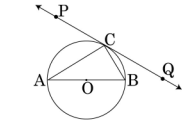
\includegraphics[width=0.6\linewidth]{1.png}
\end{center}

\item For what value of $k$ will $k+9$, $2k-1$ and $2k+7$ be the consecutive terms of an A.P.?

\item A ladder, leaning against a wall, makes an angle of $60^\circ$ with the horizontal. If the foot of the ladder is $2.5$ m away from the wall, find the length of the ladder.

\item A card is drawn at random from a well-shuffled pack of $52$ playing cards. Find the probability of getting neither a red card nor a queen.
\end{enumerate}

\section*{SECTION B}

\begin{enumerate}
\setcounter{enumi}{4}

\item If $-5$ is a root of the quadratic equation
\[
2x^2 + px - 15 = 0
\]
and the quadratic equation
\[
p(x^2 + x) + k = 0
\]
has equal roots, find the value of $k$.

\item Let $P$ and $Q$ be the points of trisection of the line segment joining the points
$A(2,-2)$ and $B(-7,4)$ such that $P$ is nearer to $A$. Find the coordinates of $P$ and $Q$.

\item In Fig., a quadrilateral $ABCD$ is drawn to circumscribe a circle with centre $O$ such that the sides $AB$, $BC$, $CD$ and $DA$ touch the circle at the points $P$, $Q$, $R$ and $S$ respectively. Prove that
\[
AB + CD = BC + DA.
\]

\begin{center}
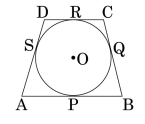
\includegraphics[width=0.6\linewidth]{2.png}
\end{center}

\item Prove that the points $(3,0)$, $(6,4)$ and $(-1,3)$ are the vertices of a right-angled isosceles triangle.

\item The 4th term of an A.P. is zero. Prove that the 25th term of the A.P. is three times its 11th term.

\item In Fig., from an external point $P$, two tangents $PT$ and $PS$ are drawn to a circle with centre $O$ and radius $r$. If $OP = 2r$, show that
\[
\angle OTS = \angle OST = 30^\circ.
\]

\begin{center}
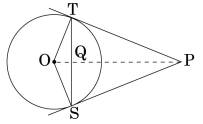
\includegraphics[width=0.6\linewidth]{3.png}
\end{center}

\end{enumerate}

\section*{SECTION C}

\begin{enumerate}
\setcounter{enumi}{10}

\item In Fig., $O$ is the centre of a circle such that diameter $AB = 13$ cm and $AC = 12$ cm. $BC$ is joined. Find the area of the shaded region.
(Take $\pi = 3.14$)

\begin{center}
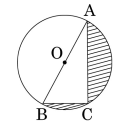
\includegraphics[width=0.6\linewidth]{4.png}
\end{center}

\item In Fig., a tent is in the shape of a cylinder surmounted by a conical top of the same diameter. If the height and diameter of the cylindrical part are $2.1$ m and $3$ m respectively and the slant height of the conical part is $2.8$ m, find the cost of canvas needed to make the tent if the canvas is available at the rate of Rs. $500$ per sq. metre.
(Use $\pi = \dfrac{22}{7}$)
\end{enumerate}

\end{document}

